\chapter{Experiments and Results}

As mentioned earlier, the work presented in this thesis is prepared on simulation and validated on real micro UAV robot. More details about the environment of the simulation is found in \ref{simu}, and about the real robot in \ref{real_robot}. An abstraction for the real robot's hardware and software specifications are mentioned in \ref{real_robot_hardware}. Robotics Operating System (ROS) has been used because of its advantages that will be discussed in section \ref{ROS_part}.

\section{Robotics Operating System} \label{ROS_part}
In the past years ROS has proved its value and grown great attention in both research and industry since it is first introduced by Andrew Ng. et al. in 2009 \cite{quigley2009ros}. It is an open source message oriented middleware with publisher subscriber message passing process. Collaborators from many companies and research laboratories develop packages and tools with the concept of being reusable. 

% some are generic with no restriction of the hardware used. 


There are now mature enough tutorials, that can give extensive and deep view of ROS like for example technical books that show step by step development using ROS as in \cite{o2014gentle,joseph2015mastering}. 



\section{Simulation} \label{simu}
There are variety of robotics simulations available in the field nowadays like MORSE, Gazebo, V-REP,Stage, etc. Available comparison about can be found examined by Gonçalo Nuno in \cite{augusto2013robotteamsim}.
\vfill
\hfill
% Some applications that utilize ROS and V-REP environment in their research as in \cite{olivares2014v}

\subsection{VREP}
Virtual Robot Experimentation Platform (V-REP) is introduced in 2013 by E. Rohmer et al. in \cite{rohmer2013v}. It has great advantage in speeding up the process of algorithm's development visualization and validation. The robot simulator V-REP, model can be individually controlled via an embedded script, a plugin, a ROS node, a remote API client, or a custom solution. This makes V-REP very versatile and ideal for multi-robot applications. Controllers can be written in C/C++, Python, Matlab, and more.
\vfill
\hfill

\subsubsection{Room}

Several rooms were built in V-REP to act as different room scenarios.

\begin{figure}
  \centering
  \subfigure[Small Room]{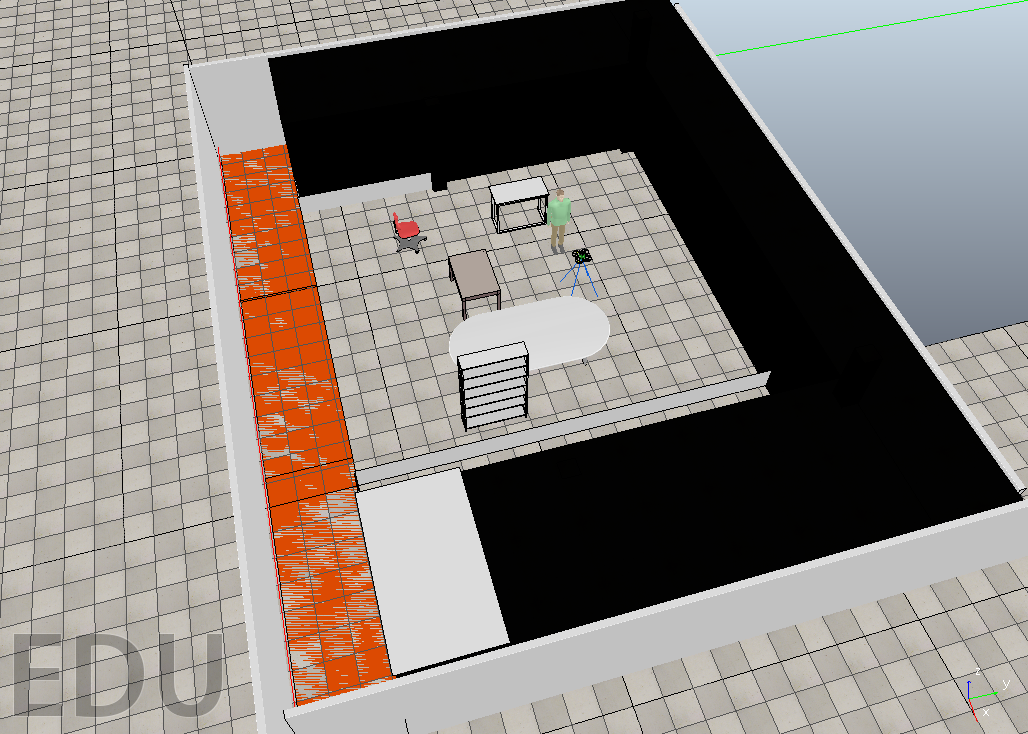
\includegraphics[width=0.45\textwidth]{figures/Room_2.png}}
  \hfill
  \subfigure[Big room]{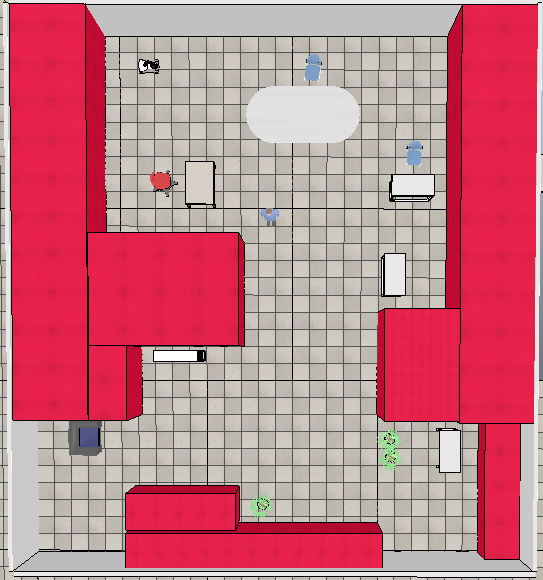
\includegraphics[width=0.45\textwidth]{figures/room_full.png}}
  \caption{Room Coverage}
  
  \label{fig:final_room}
\end{figure}

\vfill
\hfill

\subsection{UAV Simulation}
\begin{figure}[!]

  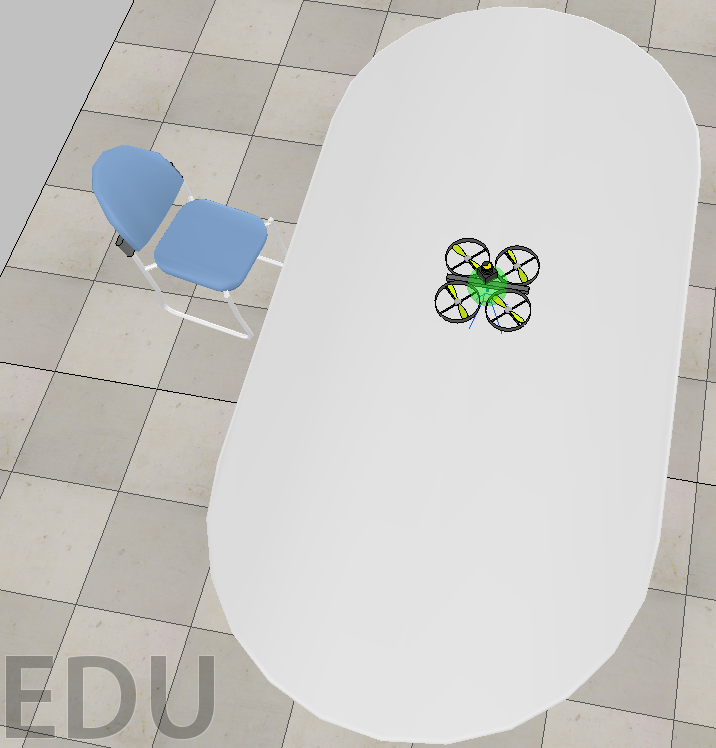
\includegraphics[width=0.5\textwidth]{figures/Drone_VREP.png}
  \caption{Drone available in V-REP with some modifications}
  
  \label{fig:drone_vrep}  
\end{figure}

\vfill
\hfill

\subsection{UAV model}

The UAV used either in simulation or real world experimentation is of micro aerial quadcopter drone like in figure \ref{fig:drone_vrep}. Obviously from the name comes quad which is equivalent to have 4 blade rotors. The quadcopter is controlled by adjusting the angular velocities of the rotors which are spun by electric motors. It has simpler structure compared to the other rotor crafts like helicopter. It can easily take off and land with vertical takeoff and landing (VTOL).  \textbf{CITE for more info}

% REF : http://sal.aalto.fi/publications/pdf-files/eluu11_public.pdf


Twist message mathematical can be found in lecture 7 graph\_slam of visual navigation for flying robots .. slide 50

\subsubsection{Mounted Camera}

There are two cameras mounted on the quadcopter available with V-REP, unfortunately their images can not be transmitted over the package used in ROS to image transport package. For this purpose editing the available model by mounting what is called according to V-REP , vision sensor. This vision sensor is giving many properties to be edited like clipping plane distance, perspective angle, resolution and more. 

% \begin{figure}
%   \centering
%   \subfigure[Small Room]{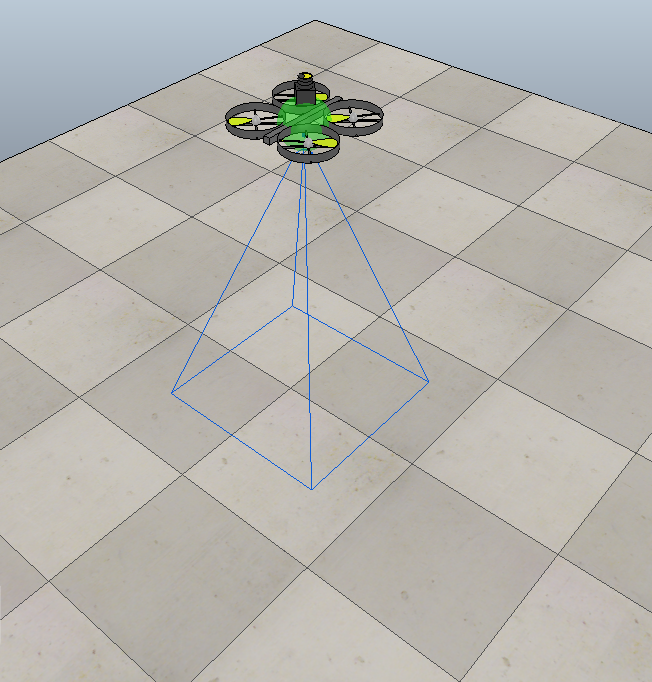
\includegraphics[width=0.23\textwidth]{figures/1m_height.png}}
%   \hfill
%   \subfigure[Big room]{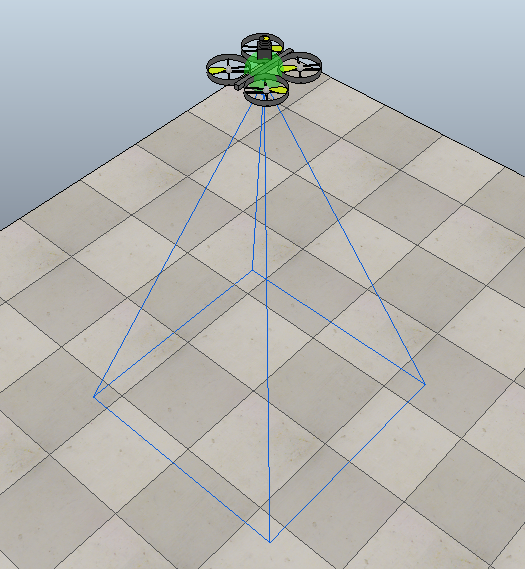
\includegraphics[width=0.23\textwidth]{figures/2m_height.png}}
  
%   \label{fig:2m_height}
%   \hfill
%   \subfigure[Big room]{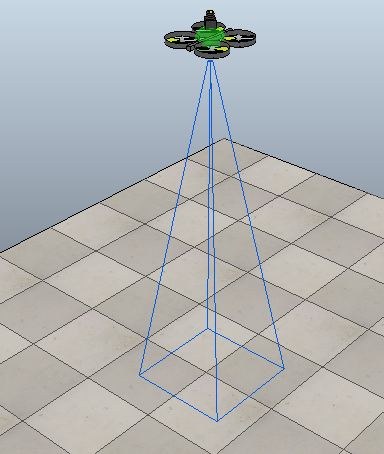
\includegraphics[width=0.23\textwidth]{figures/2m_height_small_clipping.png}}

%   \label{fig:2m_height}
  
%   \caption{Room Coverage}
% \end{figure}

% \begin{figure}[!htb]
% \minipage{0.32\textwidth}
%   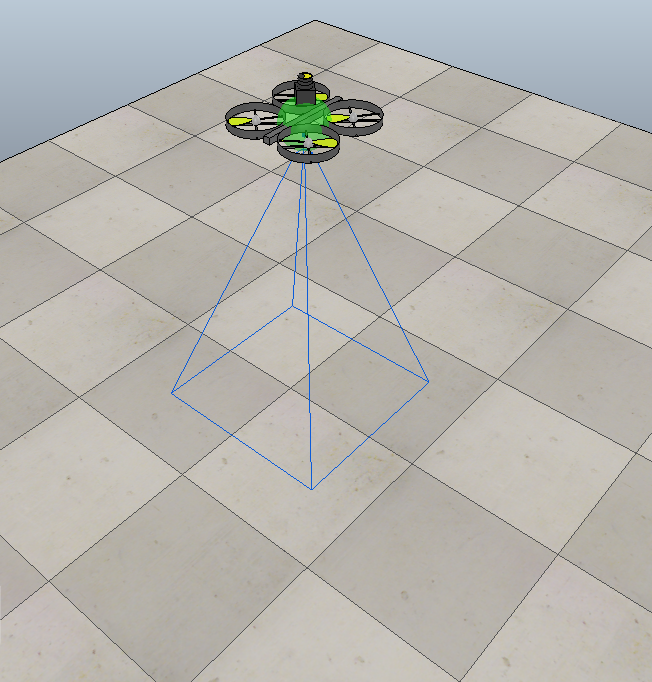
\includegraphics[width=\linewidth]{figures/1m_height.png}
%   \caption{A really Awesome Image}\label{fig:awesome_image1}
% \endminipage\hfill
% \minipage{0.32\textwidth}
%   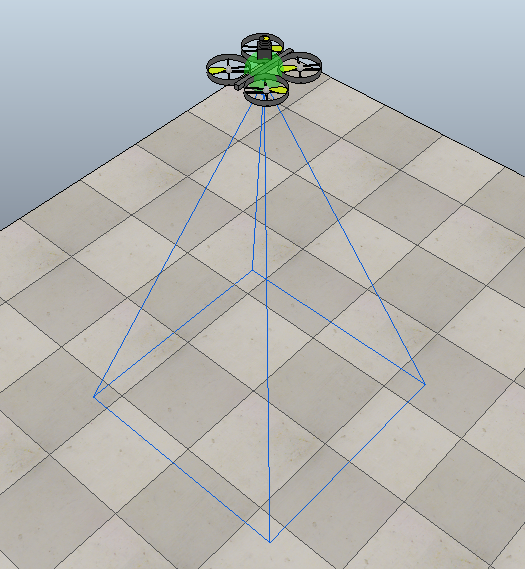
\includegraphics[width=\linewidth]{figures/2m_height.png}
% \endminipage\hfill
% \minipage{0.32\textwidth}%
%   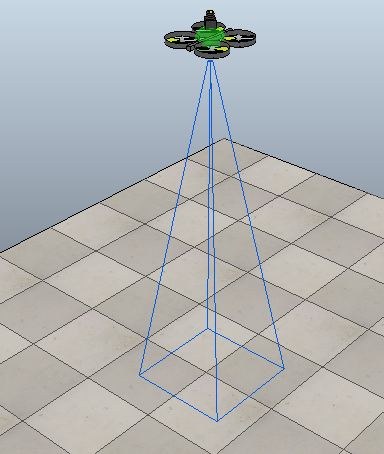
\includegraphics[width=\linewidth]{figures/2m_height_small_clipping.png}
% \endminipage
% \end{figure}

\textcolor{red}{CLEAN THE IMAGES TO BE OF THE SAME CONTOUR}

\begin{figure}[t]
\centering
\subfigure[text]{
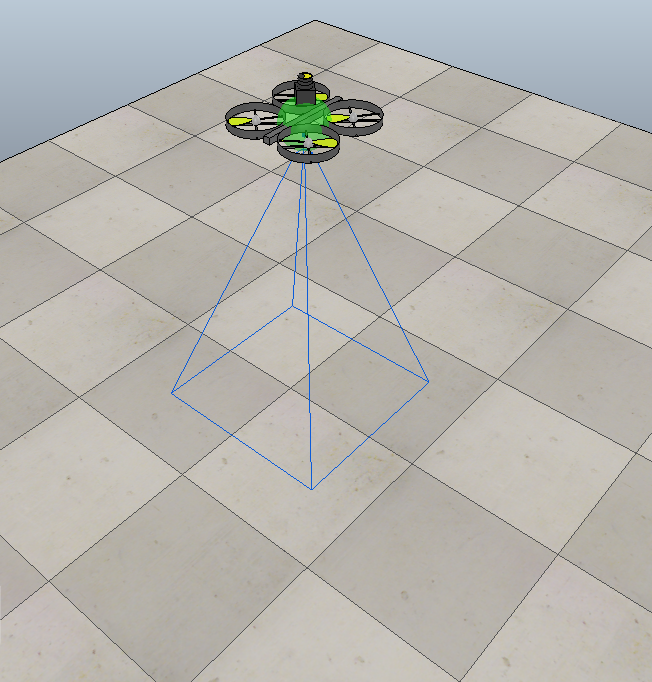
\includegraphics[width=.3\textwidth]{figures/1m_height.png}
}
\subfigure[text]{
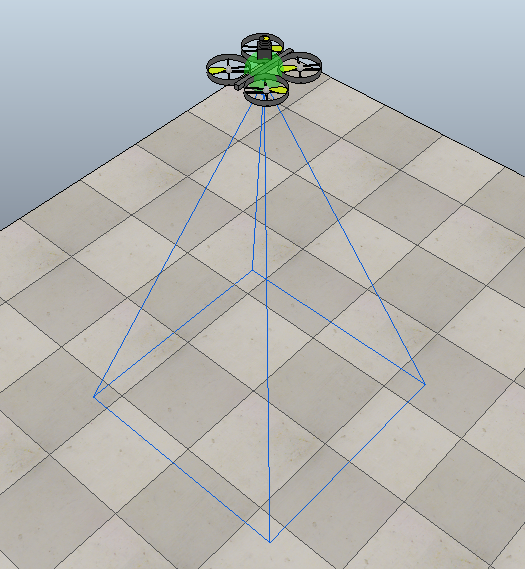
\includegraphics[width=.3\textwidth]{figures/2m_height.png}
}
\subfigure[text]{
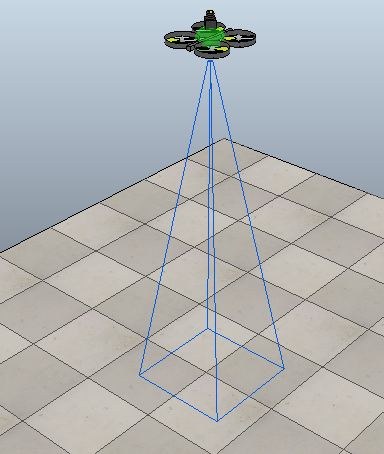
\includegraphics[width=.3\textwidth]{figures/2m_height_small_clipping.png}
}

\caption{blablabla}
\label{fig:whatever}
\end{figure}



\section{Real World Experiments} \label{real_robot}

\subsection{Quadcopter Hardware}\label{real_robot_hardware}

The Quadcoptor used to do this experiments is an offshelf commercially found drone from the French company Parrot which is AR.drone 2.0. It was first introduced in 2010 as a toy for Augmented Reality games. Shortly research labs, universities make use of its comparably cheap and low weight in their experiments. Hardware and software specification with sample research usage can be found in \cite{Ardrone1,Ardrone2}. Equipped with two cameras; one of them is pointing downwards makes it clearly very useful for the application of area coverage. This camera runs at 60 fps with a resolution of 176 x 144 pixels, covering a field of view of only 47.5$^{\circ}$ x 36.5$^{\circ}$. Concerning the software, there are mobile applications to control the drone for both IOS and Android. \textbf{SDK is avilable for computer} . The embedded software that is running onboard is not directly accessible, but sending and transmitting data with telnet shell communication channel is possible. Transmitting navigation data and receiving the sensor readings to the drone is done after connecting a workstation computer to it through ad-hoc wireless LAN network. External ROS packages used to control the quadcopter will be discussed in more details in the next subsections.


\subsection{Experiment Environment}

As mentioned in \ref{localization_Back} the wide scenarios of generating real experiments with aerial robots, localization problem is crucial. Using the monocular SLAM package developed for AR.Drone by Engel et al. in \cite{engel14ras,engel12iros}  is chosen to solve this challenge. This package proved by practical experimentation its reliability in localizing the robot without any environment modification except putting a panel full of figures to give rich features.

\textcolor{red}{put the image of the environment}


\subsection{Robot Localization }

The tum\_ardrone ROS package enables the drone to localize itself  and navigate in an unknown and potentially GPS-denied environments without learning the environment or mapping it previously. Monocular SLAM to compute a visual pose estimate within this map for each video frame. The main contribution of this package is to estimate the scale of map from inertial and altitude measurements by formulating the problem statistically, and deriving a closed-form solution for the maximum likelihood (ML) estimator of the unknown scaling factor. Proportional-integral-differential (PID) control is applied to control the pose of the drone, and fly to and hold a desired target position.


% Odometry Pose Estimation: The “Pose Estimator” is explained in the following article and Master’s Thesis [23], [22]. To correct the drift that the Odometry Pose Estimator module has, absolute measures provided by visual features are used.
 
\section{Mosaicking}
The ortho-mosaiced output image composed by the captured
images are very close to a complete top view of the area.
Mosaicing in our case is simply computed using the position and orientation coordinates of the known waypoint and stitch the images together to validate the optimum choice of the positions where the drone captured these images as shown in Fig.\ref{fig:final_room} for the simulated room in V-REP.

Otho-mosaicing also proved its validity in mosaicing aerial outdoor images as mentioned by Yahyanejad in  \cite{yahyanejad2010incremental}.

The coverage threshold rate is 90\% of the useful area in the room without taking the block parts into consideration to cover.
\hfill
\vfill

\begin{figure}[!tbp]
 \subfigure[Poses of every image captured in the room]{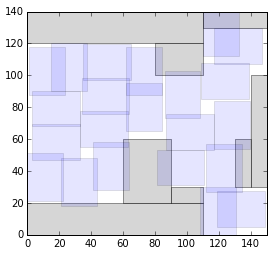
\includegraphics[width=0.45\textwidth]{figures/room_python.PNG}}
  \caption{Room Coverage}
\end{figure}

\hfill

\begin{figure}[!tbp]
  \centering
  \subfigure[Room mosaicing]{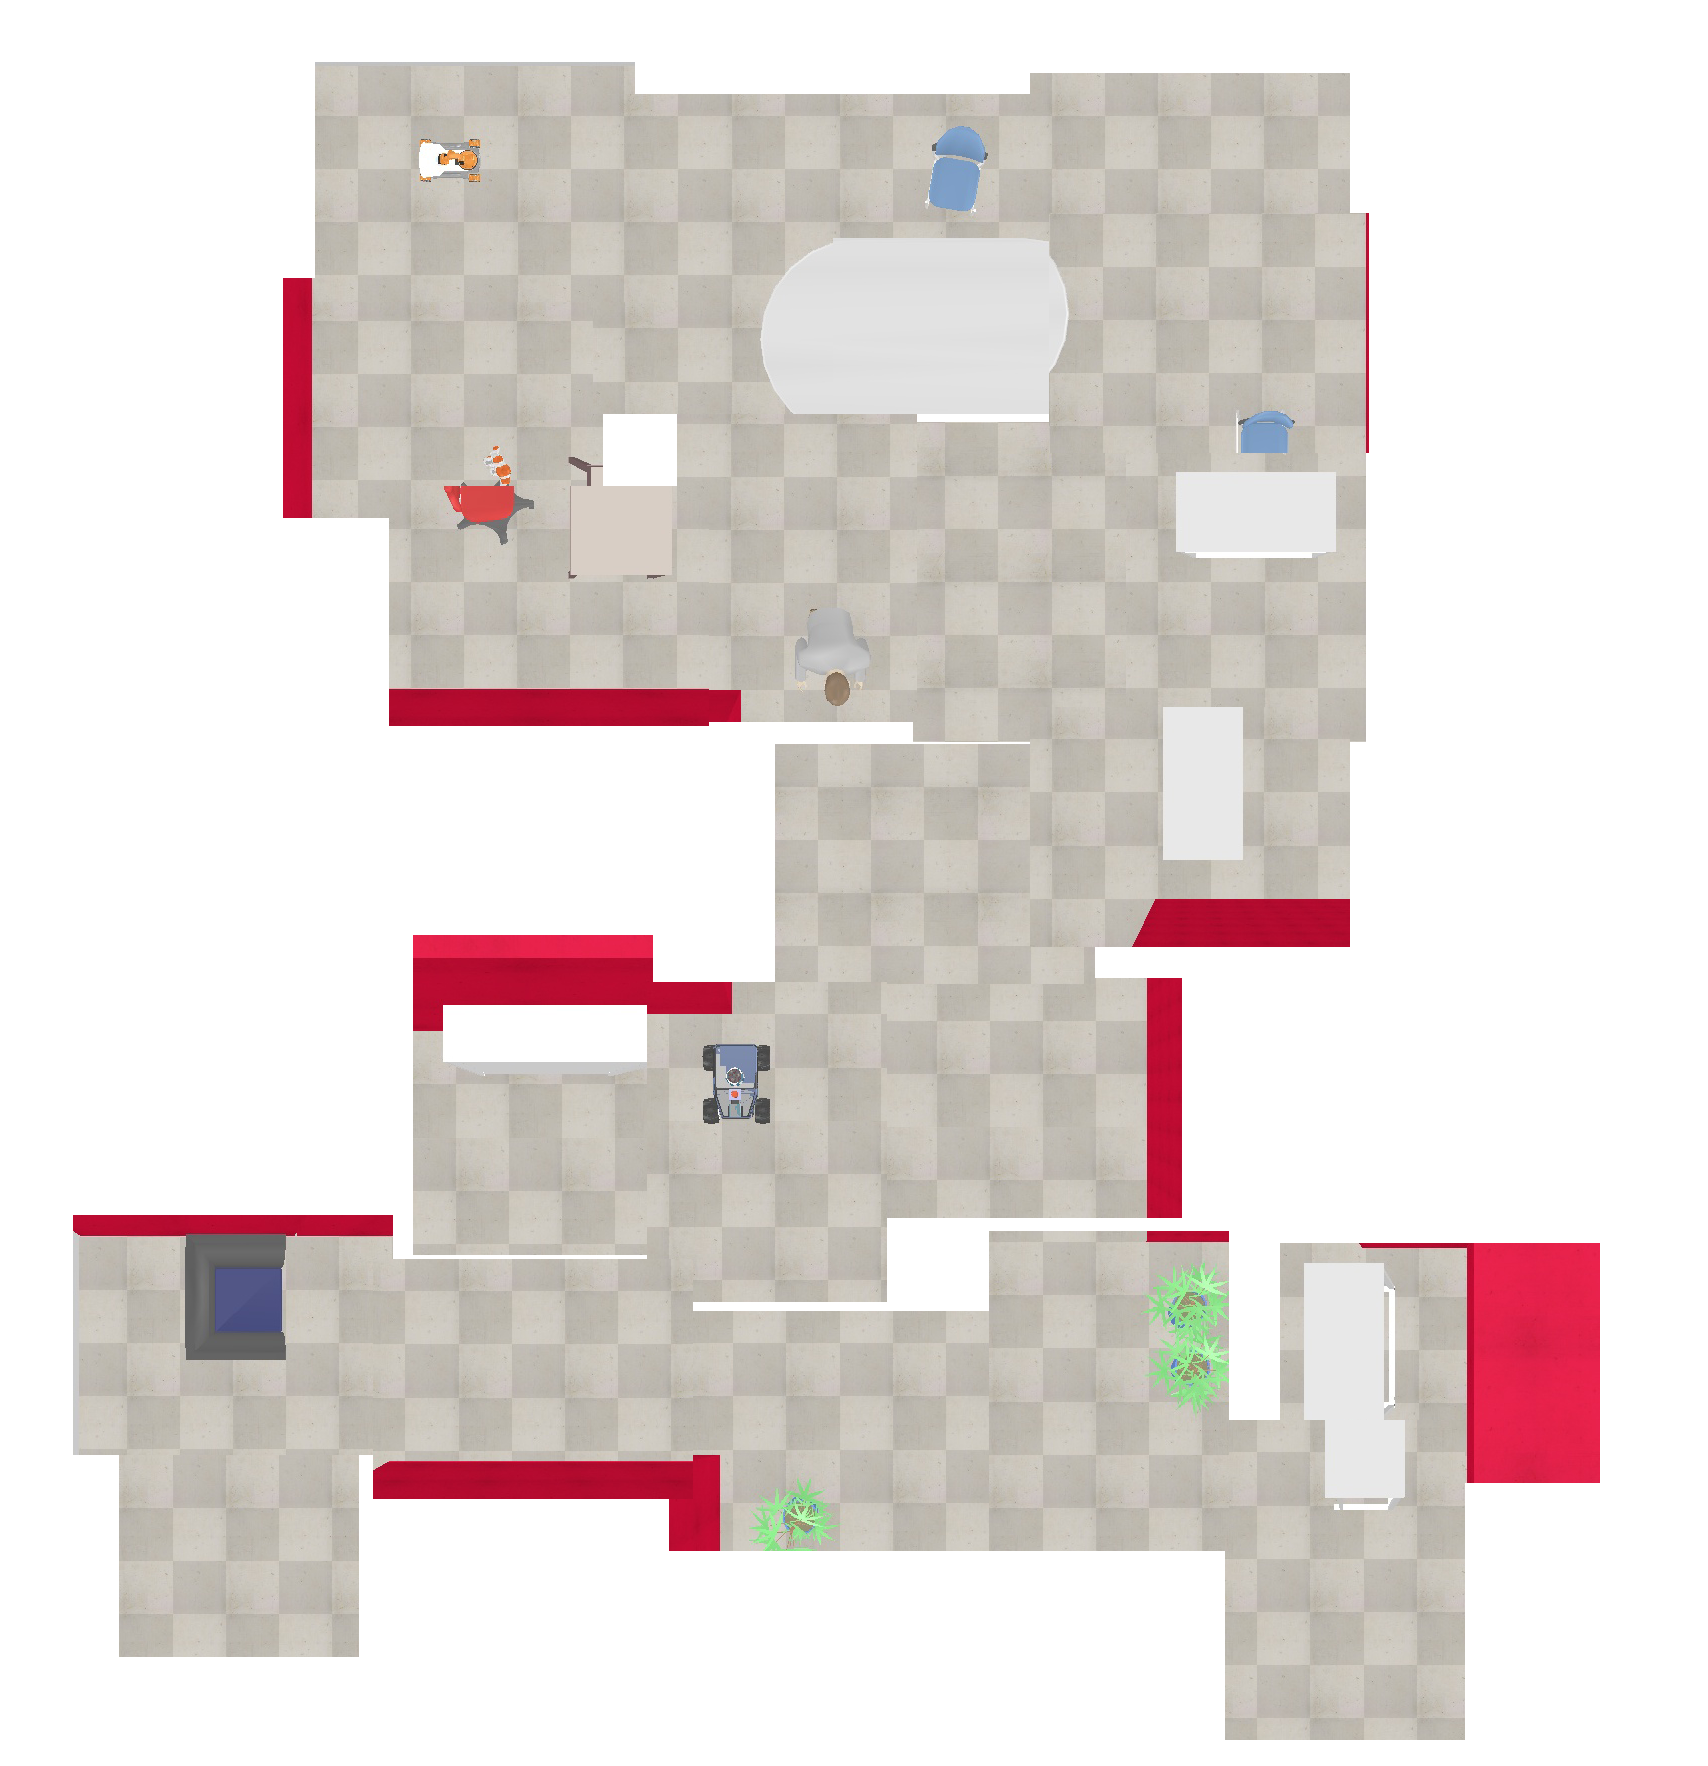
\includegraphics[width=0.45\textwidth]{figures/mosaic2.png}}
  \hfill
  \subfigure[Poses of every image captured in the room]{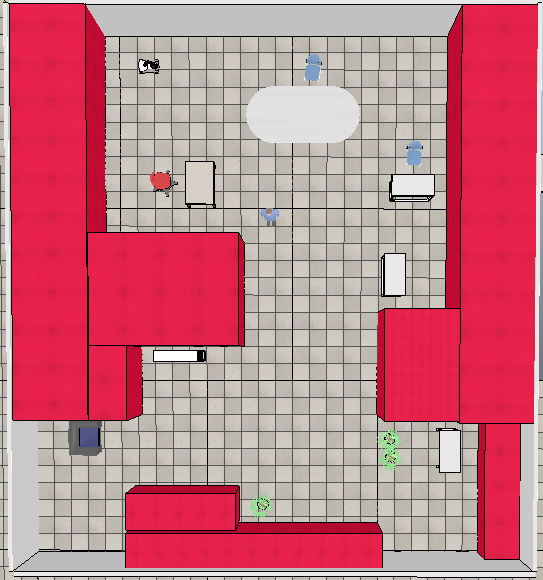
\includegraphics[width=0.45\textwidth]{figures/room_full.png}}
  \caption{Room Coverage}
  
  \label{fig:final_room}
  
\end{figure}

\hfill

\newpage

\section{Computation}
The computer used to generate these experiments is specified with 8 GB of memory (RAM). Processor is Intel® Core™ i7-2720QM CPU @ 2.20GHz ×8. 
The OS is ubuntu 14.04 LTS. Codes developed is developed by C++11, python 2, Matlab 2013B. V-REP version is 3.3.x. ROS Indigo is used.